\section{Introducción}
Google Chromecast es un dispositivo de reproducción multimedia fabricado por Google y comercializado a partir de Julio de 2013. Reproduce audio/video conectado con una televisión o monitor por HDMI haciendo streaming mediante Wi-Fi. Un nuevo modelo Chromecast Ultra que soporta 4k fue anunciado durante el evento $\#$MadeByGoogle.

Para enviar la información utiliza Google Cast, seleccionamos el contenido que queremos reproducir por una aplicación (Android 4.1+, iOS 7.0+) o mediante el navegador chrome y se carga por su puerto mico-USB.

\begin{figure*}[h]
	\centering
	\begin{minipage}[b]{.35\textwidth}
		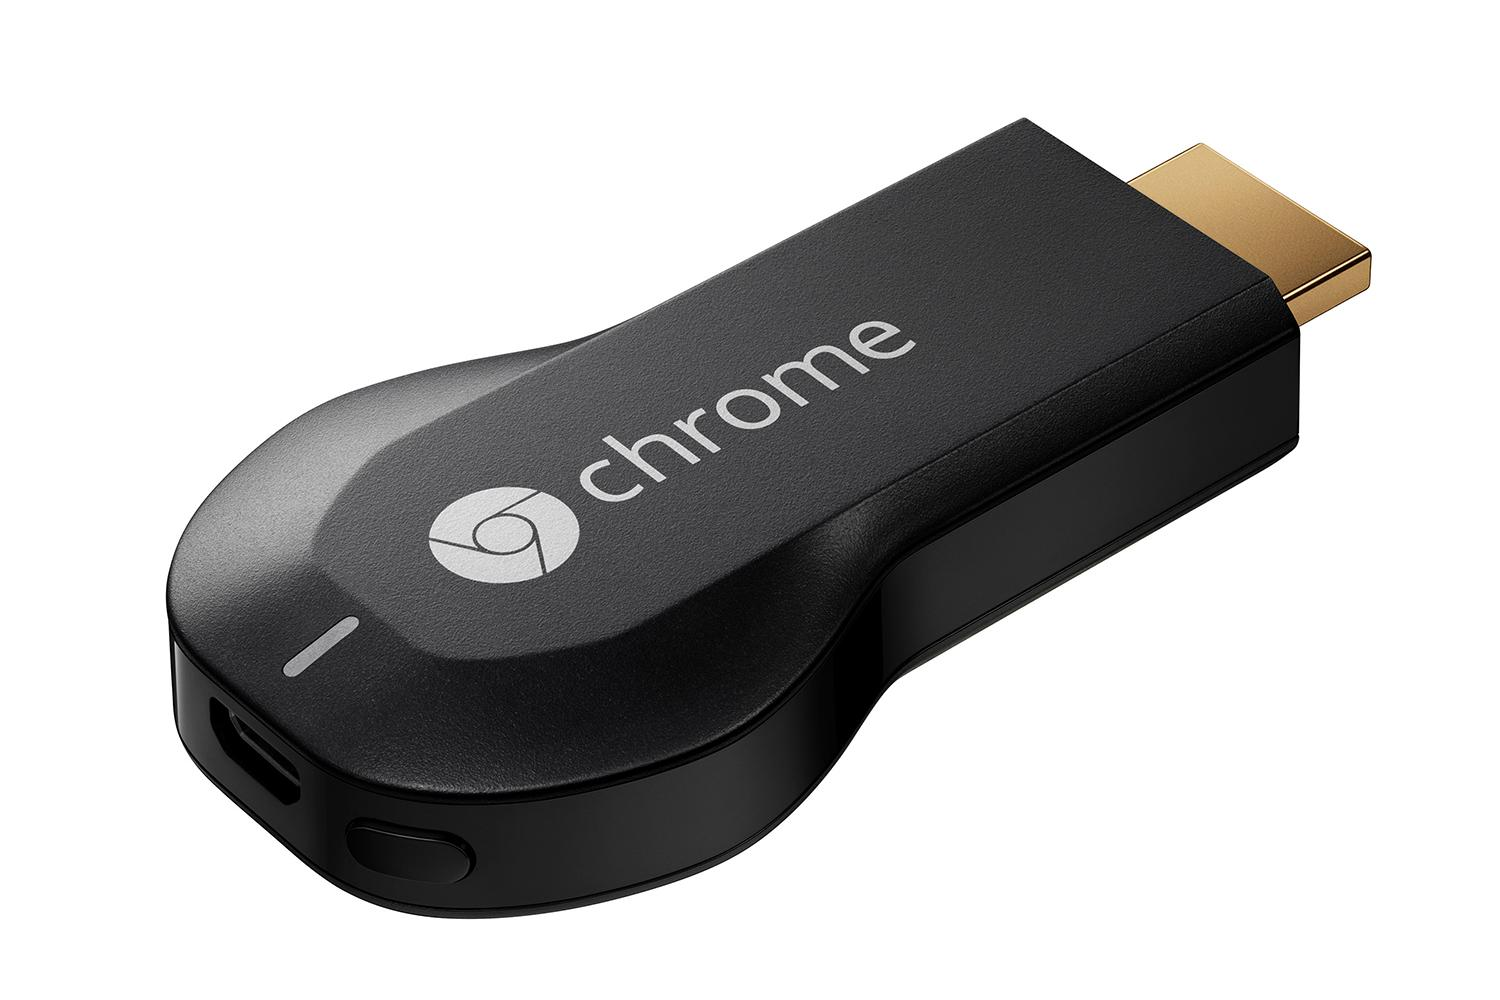
\includegraphics[scale=0.11]{./Imagenes/chromecast1gen.jpg}
		\caption{Primera generación}\label{fig:1gen}
	\end{minipage}\qquad
	\hspace{1cm}
	\begin{minipage}[b]{.35\textwidth}
		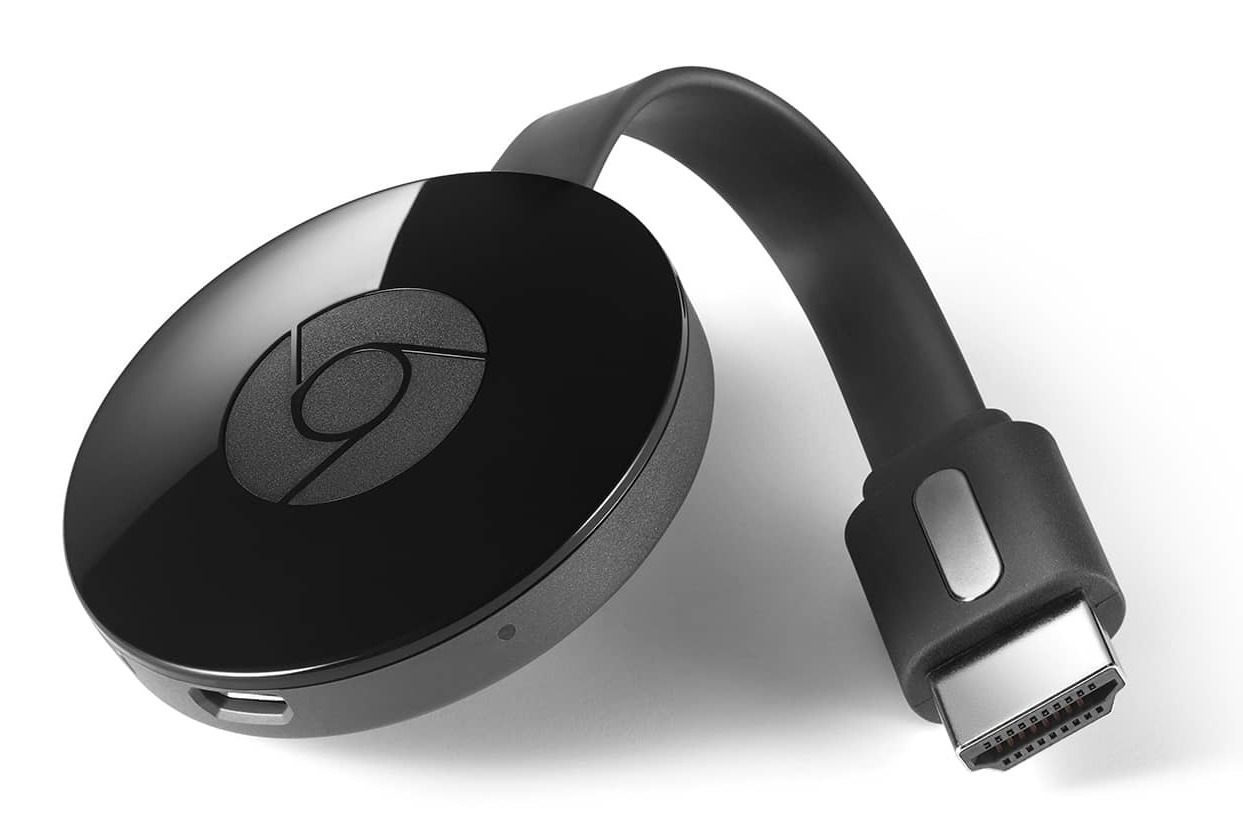
\includegraphics[scale=0.15]{./Imagenes/Chromecast.jpg}
		\caption{Segunda generación}\label{fig:2gen}
	\end{minipage}
\end{figure*}

Para iniciar la reproducción pulsamos el botón de \textit{cast}, si el puerto HDMI dispone de Consumer Electronics Control (CEC) la televisión se encenderá inmediatamente.
Dicho contenido puede residir también en su almacenamiento local. 
Con la función invitado pueden usarse redes Wi-Fi diferentes.

Las imágenes o vídeos enviados mediante dispositivos Android suelen perder calidad al estar escaladas las imágenes en pantallas pequeñas.
Cuando no hay contenido en streaming reproduce un contenido personalizable de fondo, puede incluir fotos personales, de satélite, noticias, etc.

Su principal competidor es el protocolo propietario AirPlay desarrollado por Apple Inc. que permite streaming inalámbrico entre dispositivos para audio, video, fotos, etc. 
\vspace{1cm}
\begin{figure}[h]
	\centering
	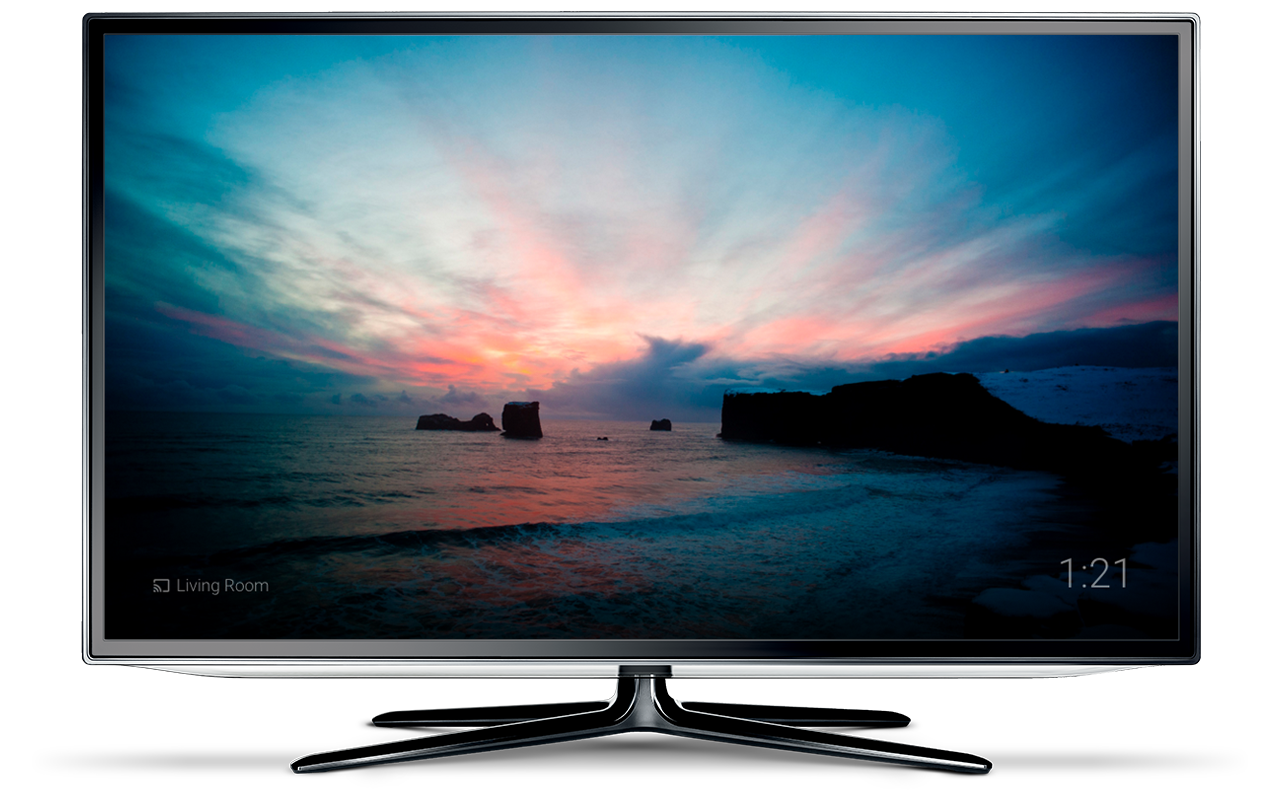
\includegraphics[width=0.6\textwidth]{./Imagenes/fondo.png}
	\label{fig:fondo}
\end{figure}

\newpage


\subsection{Generaciones}
El chromecast de primera generación incluye un decodificador de VP8 y H.264 para formatos de compresión de vídeo, 512 MB de Micron DDR3L RAM y 2 GB de memoria flash.
El de segunda generación tiene un cable flexible y magnético, usa procesador dual ARM Cortex-A7 de frecuencia 1.2 GHz y tiene tres antenas adaptativas para mejroar la conexión con el router.
El dispositivo tiene 512 MB de Samsung DDR3L RAM y 256 MB de memoria flash.